

\documentclass[sigconf]{acmart}

\usepackage[english]{babel}
\usepackage{blindtext}

% Copyright
\renewcommand\footnotetextcopyrightpermission[1]{} % removes footnote with conference info
\setcopyright{none}
%\setcopyright{acmcopyright}
%\setcopyright{acmlicensed}
%\setcopyright{rightsretained}
%\setcopyright{usgov}
%\setcopyright{usgovmixed}
%\setcopyright{cagov}
%\setcopyright{cagovmixed}

\settopmatter{printacmref=false, printccs=false, printfolios=true}

% DOI
\acmDOI{}

% ISBN
\acmISBN{}

%Conference
%\acmConference[Submitted for review to SIGCOMM]{}
%\acmYear{2018}
%\copyrightyear{}

%% {} with no args suppresses printing of the price
\acmPrice{}

\usepackage{multirow}  % Add this in your preamble


\usepackage{color}
\usepackage{tikz}
\usepackage[tight]{subfigure}
\usepackage{comment}
\usepackage{amsmath}
\usepackage{enumerate}
\usepackage{multirow}
\usepackage{hhline}

\usepackage{enumerate}
\usepackage{enumitem}

\usepackage{xurl}       % better URL line breaking
\usepackage{hyperref}   % hyperlinks (loads url automatically)


\usepackage{slashbox}

\usepackage{amsmath}
\usepackage{xspace}
\usepackage{algorithm}
\usepackage[font=small]{caption}
\usepackage[noend]{algpseudocode}
\usepackage[capitalize]{cleveref}
\makeatletter
\def\BState{\State\hskip-\ALG@thistlm}
\makeatother

\algdef{SE}[SUBALG]{Indent}{EndIndent}{}{\algorithmicend\ }%
\algtext*{Indent}
\algtext*{EndIndent}
\algrenewcommand\algorithmicindent{1.0em}%

\usepackage[normalem]{ulem}
\usepackage{subcaption}
\usepackage[english]{babel}
\usepackage{amsmath}
\usepackage{xspace}
\usepackage{booktabs}
\usepackage{tabularx}
\usepackage{enumitem}
\usepackage{tikz}
\usetikzlibrary{arrows.meta,positioning,fit,shapes.geometric}
\usepackage[font=small]{caption}
\usepackage{xurl}
\usepackage{balance}

%%%% remove all comments?
\newif\ifcomm
\commtrue
\ifcomm
\else
\commfalse
\fi
\ifcomm
	\newcommand{\mycomm}[3]{{\footnotesize{{\color{#2} \textbf{[#1: #3]}}}}}
    \newcommand{\revise}[1]{\textcolor{purple}{\textbf{#1}}}
    \newcommand{\removeold}[1]{}
    \newcommand{\remove}[1]{\textcolor{orange}{\textbf{#1}}}
\else
    \newcommand{\mycomm}[3]{}
    \newcommand{\revise}[1]{#1}
    \newcommand{\removeold}[1]{}
    \newcommand{\remove}[1]{}
\fi


\newcommand{\MM}[1]{\mycomm{MM}{red}{#1}}  
\newcommand{\ran}[1]{\mycomm{Ran}{blue}{#1}}
\newcommand{\shay}[1]{\mycomm{Shay}{red}{#1}}
\newcommand{\Wenchen}[1]{\mycomm{Wenchen}{Wenchen}{#1}}



\newcommand{\norm}[1]{\left\lVert#1\right\rVert}
\newcommand{\E}{\mathbb{E}}
\newcommand{\floor}[1]{\left\lfloor#1\right\rfloor}
\newcommand{\ceil}[1]{\left\lceil#1\right\rceil}
\newcommand{\parentheses}[1]{\left(#1\right)}
\newcommand{\angles}[1]{\left\langle#1\right\rangle}
\newcommand{\brackets}[1]{\left[#1\right]}
\newcommand{\set}[1]{\left\{#1\right\}}
\newcommand{\abs}[1]{\left|#1\right|}
\newcommand{\indicator}{\ensuremath{\mathbb{1}}}
\newcommand{\sbrac}[1]{\left[ #1 \right]}
%\newcommand{\para}[1]{\left( #1 \right)} 
\newcommand{\Var}[1]{\mathrm{Var}{#1}} 
\newcommand{\nqv}{\ensuremath{s}}


\definecolor{Wenchen}{RGB}{200,0,200}

% \usepackage{titlesec}
%\setlength{\abovedisplayskip}{-35pt}
%\setlength{\belowdisplayskip}{-35\pt}
%\setlength{\abovedisplayshortskip}{-35pt}
%\setlength{\belowdisplayshortskip}{-35pt}
\setlength{\textfloatsep}{3pt}% Reduce \textfloatsep
% \titlespacing\section{0pt}{6pt plus 4pt minus 2pt}{5pt plus 2pt minus 2pt}
% \titlespacing\subsection{0pt}{6pt plus 4pt minus 2pt}{5pt plus 2pt minus 2pt}
% \titlespacing\subsubsection{0pt}{6pt plus 4pt minus 2pt}{5pt plus 2pt minus 2pt}


\hypersetup{pdfstartview=FitH,pdfpagelayout=SinglePage}

% \setlength\paperheight {11in}
% \setlength\paperwidth {8.5in}
% \setlength{\textwidth}{7in}
% \setlength{\textheight}{9.25in}
% \setlength{\oddsidemargin}{-.25in}
% \setlength{\evensidemargin}{-.25in}

\newcommand{\ppp}{\noindent\textbf}
\newcommand{\subp}{\noindent\textbf}
\newcommand{\bbb}{\noindent\textif}

\newcommand{\ie}{\textit{i.e.}}
\newcommand{\eg}{\textit{e.g.}}
\newcommand{\para}[1]{\noindent{\bf #1} }

\newcommand{\sysname}{\textsc{PRED-MoE}\xspace}
\newcommand{\sys}{\sysname}


\renewcommand{\eg}{e.g.}

\begin{document}
\title[POSTER: \sysname]{POSTER: Prediction-Enhanced Expert Prefetching and Eviction for MoE Offloading via \sysname}


%\titlenote{Produces the permission block, and copyright information}
%\subtitle{Extended Abstract}

\author{Wenchen Han}
\affiliation{%
  \institution{University College London}%
  % \city{London}
  \country{}%  
}

\author{Shay Vargaftik} 
\affiliation{%
  \institution{VMware Research by Broadcom}%
  \country{}%  
}

\author{Michael Mitzenmacher}
\affiliation{%
  \institution{Harvard University}%
  \country{}%  
}

%\authornote{Michael Mitzenmacher was supported in part by NSF grants CCF-2101140, CNS-2107078, and DMS-2023528.
%}



\author{Ran Ben Basat}
\affiliation{%
  \institution{University College London}%
  % \city{London}
  \country{}%  
}  

\renewcommand{\shortauthors}{W. Han, S. Vargaftik, M. Mitzenmacher, R. Ben Basat}

\begin{abstract}
Mixture-of-Experts (MoE) models improve scaling by activating a small number of experts per token. 
However, the combined memory requirements of all experts may exceed the available GPU high bandwidth memory (HBM) during serving. 
Inference frameworks such as vLLM and HuggingFace address the problem by offloading inactive experts to CPU memory and moving them to the GPU's HBM as needed. While enabling inference of large models on limited HBM setups, this CPU-GPU traffic overhead slows token generation speed substantially.

We present \sys, a correctness-preserving prefetching and eviction policy for MoE offloading. 
\sys leverages a lightweight predictor to assess which experts assess which experts are most likely to be required for prefetching and ranks experts by their likelihood of near-future for eviction. Preliminary evaluation over the Qwen3-30B-A3B model and the MMLU-Pro dataset indicates that \sys reduces the TPOT of vLLM and HuggingFace by up to $3.02\times$ and $28.62\times$ respectively.
\end{abstract}

\maketitle

\section{Introduction}
MoE layers route each token to a small subset of experts, enabling larger parameter counts for the same HBM size~\cite{shazeer2017outrageously,fedus2022switch,jiang2024mixtral}. The challenge in serving MoE models is that expert parameters dominate the memory footprint: a model may compute with only a few experts at any time, but the full set of experts must be resident somewhere. When the active expert set does not fit in GPU memory, a common solution is \emph{MoE offloading}: keep only a subset of experts on the GPU and store the rest in CPU memory, loading experts on demand.  
This extensive CPU-GPU traffic overhead slows down and often dominates the token generation speed. 

Intuitively, one can view this as a prefetching-caching problem. The system is allowed to prefetch experts that are likely to be useful in the near future, and an eviction policy dictates which experts to replace to make room when needed.
Importantly, the cache miss penalty is high because a miss stalls the MoE layer until expert weights arrive over the CPU--GPU interconnect. 

Prior systems demonstrate the promise of expert offloading, prefetching, and predictive routing \cite{eliseev2023fast,du2024sida,he2026expertflow}, but the eviction decision itself often overlooks the problem's auto-regressive nature or may negatively alter system behavior (e.g., by modifying expert selection). 

To address this gap, we profile and characterize expert activation patterns and use our findings to construct a real-time, lightweight predictor that assigns each expert a likelihood of being required in the near future. We design \sys, a prediction-based prefetching and eviction framework that ensures correctness by serving the exact set of experts selected by the router while minimizing CPU-GPU traffic overhead to improve generation speed.

We conducted a preliminary evaluation with the Qwen3-30B-A3B model~\cite{qwen2025qwen330ba3b} on the MMLU-Pro dataset~\cite{wang2024mmlupro}. Results show that under varying GPU memory size and batch size up to $64$, \sysname outperforms vLLM~\cite{kwon2023vllm} and HuggingFace~\cite{wolf2019huggingface} by $2.26\sim 3.02\times$ and $18.23 \sim 28.62\times$ respectively.


\section{\sysname Design}
\subsection{Problem formulation}
We formulate MoE offloading as an online prefetching and caching problem.
The GPU stores a subset of expert weights, while CPU memory stores a
copy of every expert. The goal of \sys is not to change the model's
routing decisions, but to ensure that the experts selected by the original
router are already resident on GPU when they are needed.


Let $\mathcal{L}$ be the set of MoE layers. 
Each layer $\ell\in\mathcal{L}$ contains a set of experts $\mathcal{E}_\ell$, where the sets are disjoint.
The set of all experts in the model is
$\mathcal{X}=\bigcup_\ell \mathcal{E}_\ell$.
During autoregressive decoding, let $\mathcal{T}$ be the set of generation
steps, and let $t\in\mathcal{T}$ denote one such step. The first generated token
corresponds to the first element of $\mathcal{T}$. Let $\mathcal{B}_t$ be the
set of active requests at generation step $t$.

For each active request $b\in\mathcal{B}_t$, layer $\ell\in\mathcal{L}$, and
generation step $t\in\mathcal{T}$, the router selects a small subset of experts:
$\mathcal{A}_{b,t,\ell}\subseteq \mathcal{E}_\ell$.
The batch-level active expert set for layer $\ell$ at step $t$ is $\mathcal{A}_{t,\ell}=\bigcup_{b\in\mathcal{B}_t}\mathcal{A}_{b,t,\ell}$.

Let $\mathcal{C}^{-}_{t,\ell}\subseteq\mathcal{X}$ denote the set of experts
resident in GPU memory immediately before the expert computation of layer $\ell$ at
step $t$. This state is measured after completing
prefetches but before loading any expert that is required and is missing, i.e., $\mathcal{A}_{t,\ell}\setminus \mathcal{C}^{-}_{t,\ell}$ is the set of experts that must be loaded before the layer can process the batch. 
Therefore, any expert
$x\in \mathcal{A}_{t,\ell}\setminus \mathcal{C}^{-}_{t,\ell}$ 
must load from CPU memory. Such a cache
miss preserves model correctness, but increases~latency.

After the current layer's expert computation begins, the system may prefetch
experts that it predicts will be useful in future layer-step pairs
$(t',\ell')$. When the cache exceeds its capacity $C$, the eviction policy chooses
inactive resident experts to remove. Experts currently participating in the
layer computation may not be replaced by the prefetched~experts.
Our goal is to minimize the miss-induced transfer time:
\begin{equation*}
\label{eq:cache-objective}
\min_{\pi}\;
\sum_{t\in\mathcal{T}}
\sum_{\ell\in\mathcal{L}}
\sum_{x\in\mathcal{A}_{t,\ell}}
w_x \cdot \left(x\notin\mathcal{C}^{-}_{t,\ell}\right),
\quad
\text{s.t.}\quad
|\mathcal{C}_{t,\ell}|\le C .
\end{equation*}



Here, $w_x$ is the blocking transfer cost of loading expert $x$ from CPU memory
to GPU memory. If we assume, as we do henceforth, that all experts have the same size and use the same transfer
path, so $w_x$ is constant, the objective reduces to minimizing the number of
expert cache misses.

This objective intentionally abstracts away two lower-level effects. First,
expert loads may have different costs depending on expert size, GPU placement,
interconnect bandwidth, and whether the load is local or remote; these effects
can be modeled by choosing nonuniform weights $w_x$. Second, the objective does
not charge a separate cost for prefetched experts that are not immediately used.
This is a reasonable approximation when prefetch traffic is bounded and overlaps
with current-layer computation. False prefetches are not completely free,
however: they still consume cache capacity and can indirectly increase future
misses by evicting useful experts. We intend to explore such advanced modeling as varying $w_x$ or charging prefetch bandwidth in future work.

\subsection{Expert activation patterns}\label{sec:expert_activation_patterns}

\sys utilizes three properties of MoE routing, aligning with \mbox{observations from previous work (e.g., ~\cite{wang2025harnessing, zhou2022mixture}).}
First, by design, for each request and layer, the router usually activates only a small, usually fixed-size,
subset of the layer's experts:
$
\mathcal{A}_{b,t,\ell}\subseteq \mathcal{E}_\ell$, where $|\mathcal{A}_{b,t,\ell}| \ll |\mathcal{E}_\ell|$. 
Moreover, routing is often skewed, where many requests in the same batch select
overlapping experts. As a result, the batch-level active set
$\mathcal{A}_{t,\ell}$ is often much smaller than the full expert set of layer $\ell$: $|\mathcal{A}_{t,\ell}| \ll |\mathcal{E}_\ell|$.
This concentration occurs because popular experts may be selected by many tokens
in the batch, while rarely used experts are selected by few or no tokens.

Second, decode steps often exhibit temporal locality. For a fixed layer
$\ell\in\mathcal{L}$, the active set at a generation step often overlaps with the
active sets observed at nearby steps. Informally,
$\mathcal{A}_{t,\ell}$ is predictive of the active sets that will appear in the future. 
This makes recent expert usage a useful signal for eviction:
experts used recently are more likely to be reused than experts which have been inactive. 

Third, expert choices are token- and context-dependent. The router's decisions
are correlated with the token representation being processed, and therefore with
features of the current request and generation state. \sys uses profiling to
learn these correlations and predict which experts are likely to be needed in
upcoming layers or decode steps.

Together, these properties suggest a prediction-enhanced eviction policy: keep
experts that are likely to be reused soon, prefetch experts predicted for future
layer-step pairs, and evict inactive experts with low predicted reuse
probability.

\subsection{Prefetching and eviction}

At each step $t$ and MoE layer $\ell$, \sys performs four steps. (1) Run the router and compute $\mathcal{A}_{t,\ell}$.
(2) If capacity is lower than $\mathcal{A}_{t,\ell}\setminus \mathcal{C}^{-}_{t,\ell}$, protect the current active set and select eviction victims from the lowest-score inactive experts. (3) Admit every expert in $\mathcal{A}_{t,\ell}\setminus \mathcal{C}^{-}_{t,\ell}$ by CPU-to-GPU copy, overlapping copies with non-expert work when possible. (4) Update the routing trace and predictor features (i.e., we employ online training to preserve accuracy as workloads change). (5) \textit{While the current batch is being processed by this layer,} select experts to pre-fetch to optimize future steps/layers; select eviction victims; and replace them with additional CPU-to-GPU copying. 

\MM{I feel like we've really inflated the idea of prefetch+eviction, and then in evaluation we don't do prefetch.
I think we need to say that earlier (intro) and repeat it here at the very start of the evaluation section, or it looks like we're burying it.}

\section{Evaluation}
Our preliminary implementation of \sysname consists of two core components: an MoE offloading engine implemented atop vLLM~\cite{kwon2023vllm} that manages the prefetching-caching during inference and a lightweight predictor module, being trained offline in our prototype, that ranks experts according to the likelihood they will be needed in the next few steps. 

\begin{figure}[h!]
    \centering
    \vspace{0.1in}
    \hspace{-0.15cm}
    \subfigure[TPS w.r.t. GPU memory usage]{
        \begin{minipage}[t]{0.48\linewidth}{
        \vspace{-0.00in}
        \begin{center}
        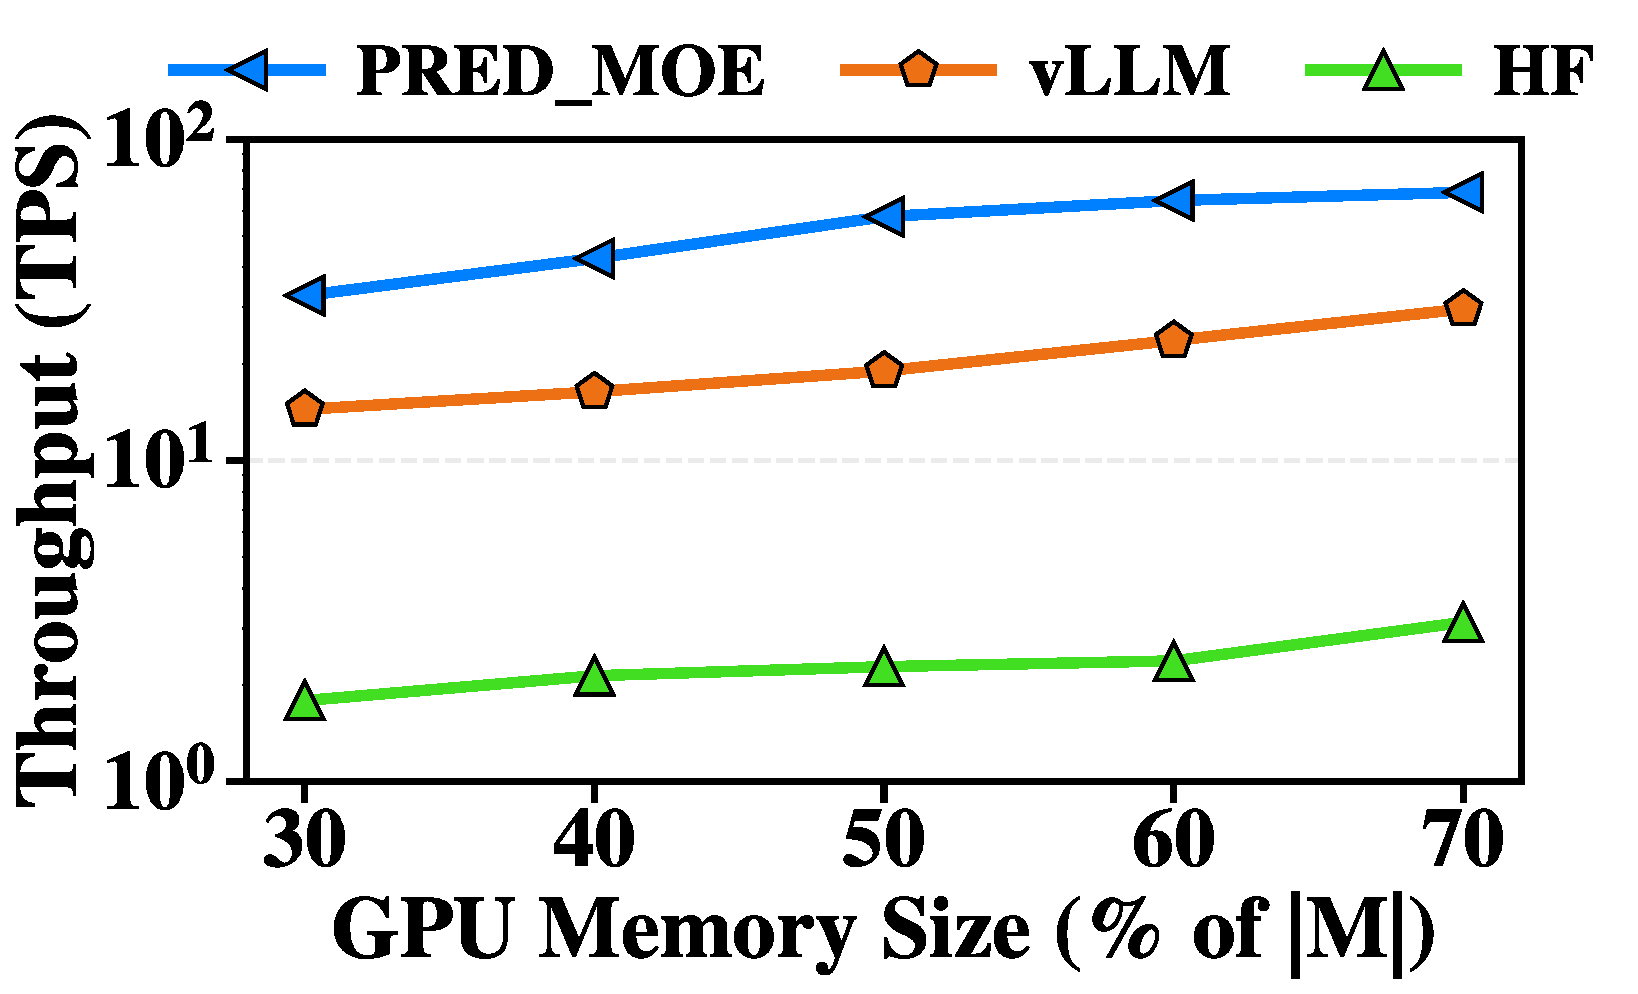
\includegraphics[width=\textwidth]{figures/poster_tps_vs_gpu_memory.pdf}
        \end{center}
        \vspace{-0.1cm}
        }
        \label{subfig:tps-vs-gpu-memory}
        \end{minipage}
    }
    %
    \hspace{-0.1cm}
    \subfigure[TPS w.r.t. batch size]{
        \begin{minipage}[t]{0.48\linewidth}{
        \vspace{-0.00in}
        \begin{center}
        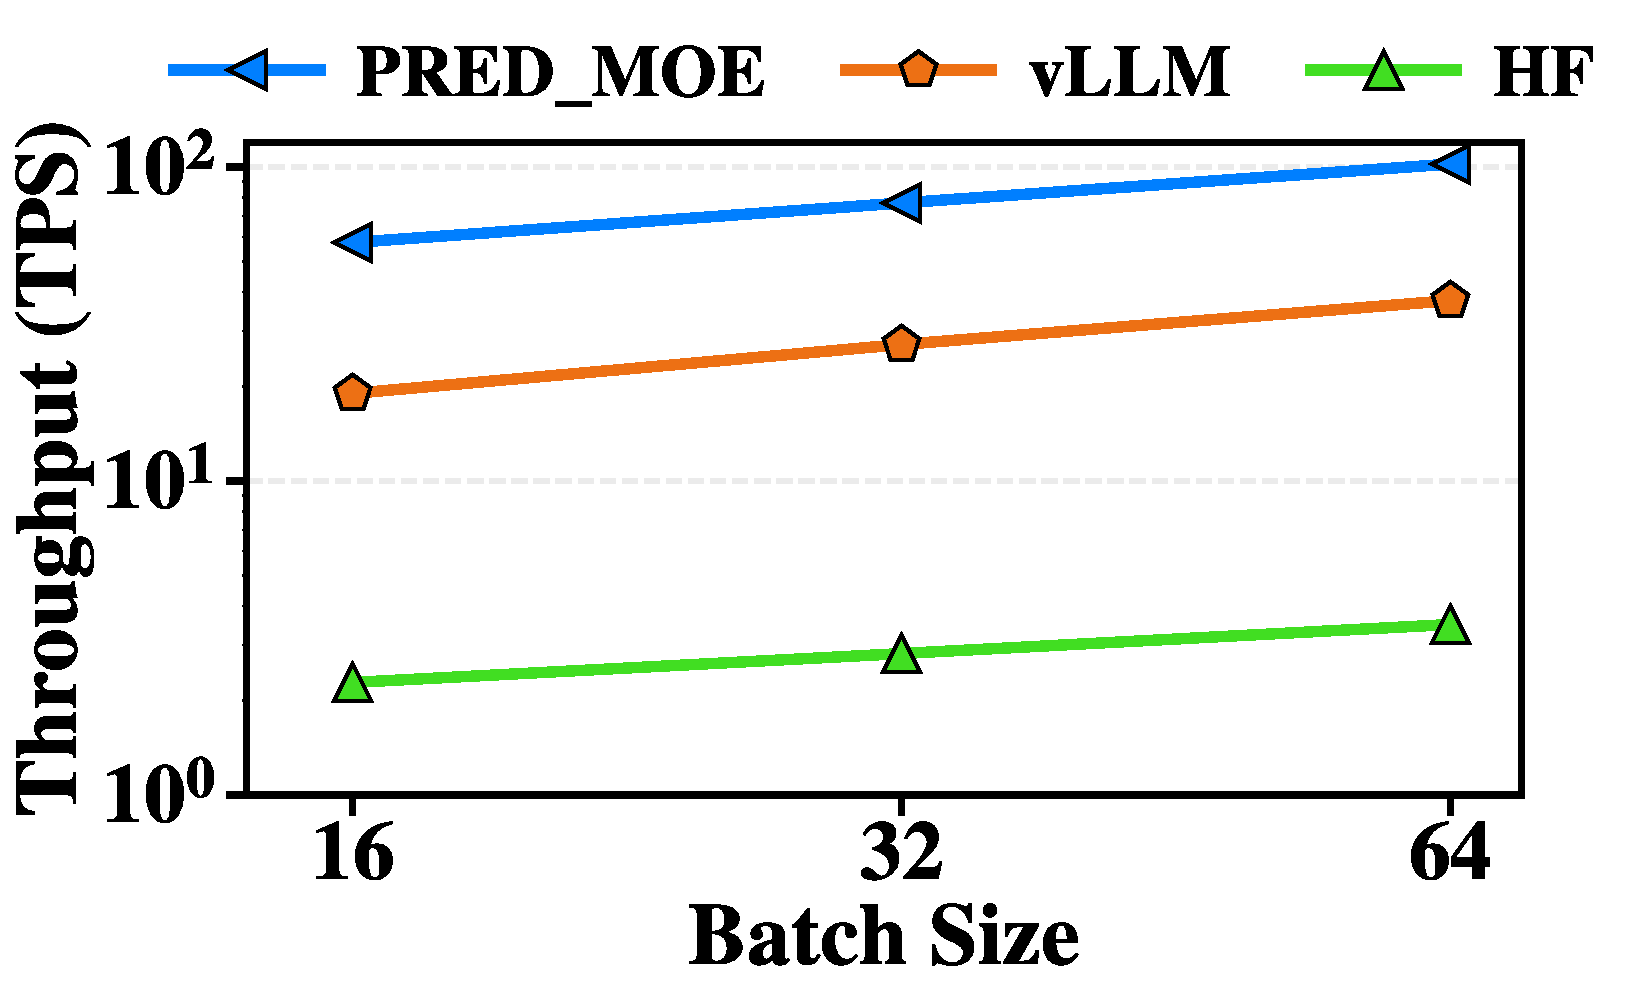
\includegraphics[width=\textwidth]{figures/poster_tps_vs_batch_size.pdf}
        \end{center}
        \vspace{-0.1cm}
        }
        \label{subfig:tps-vs-batch-size}
        \end{minipage}
    }

    \vspace{-0.3cm}
    \subfigure[TPOT w.r.t. GPU memory usage]{
        \begin{minipage}[t]{0.475\linewidth}{
        \vspace{-0.00in}
        \begin{center}
        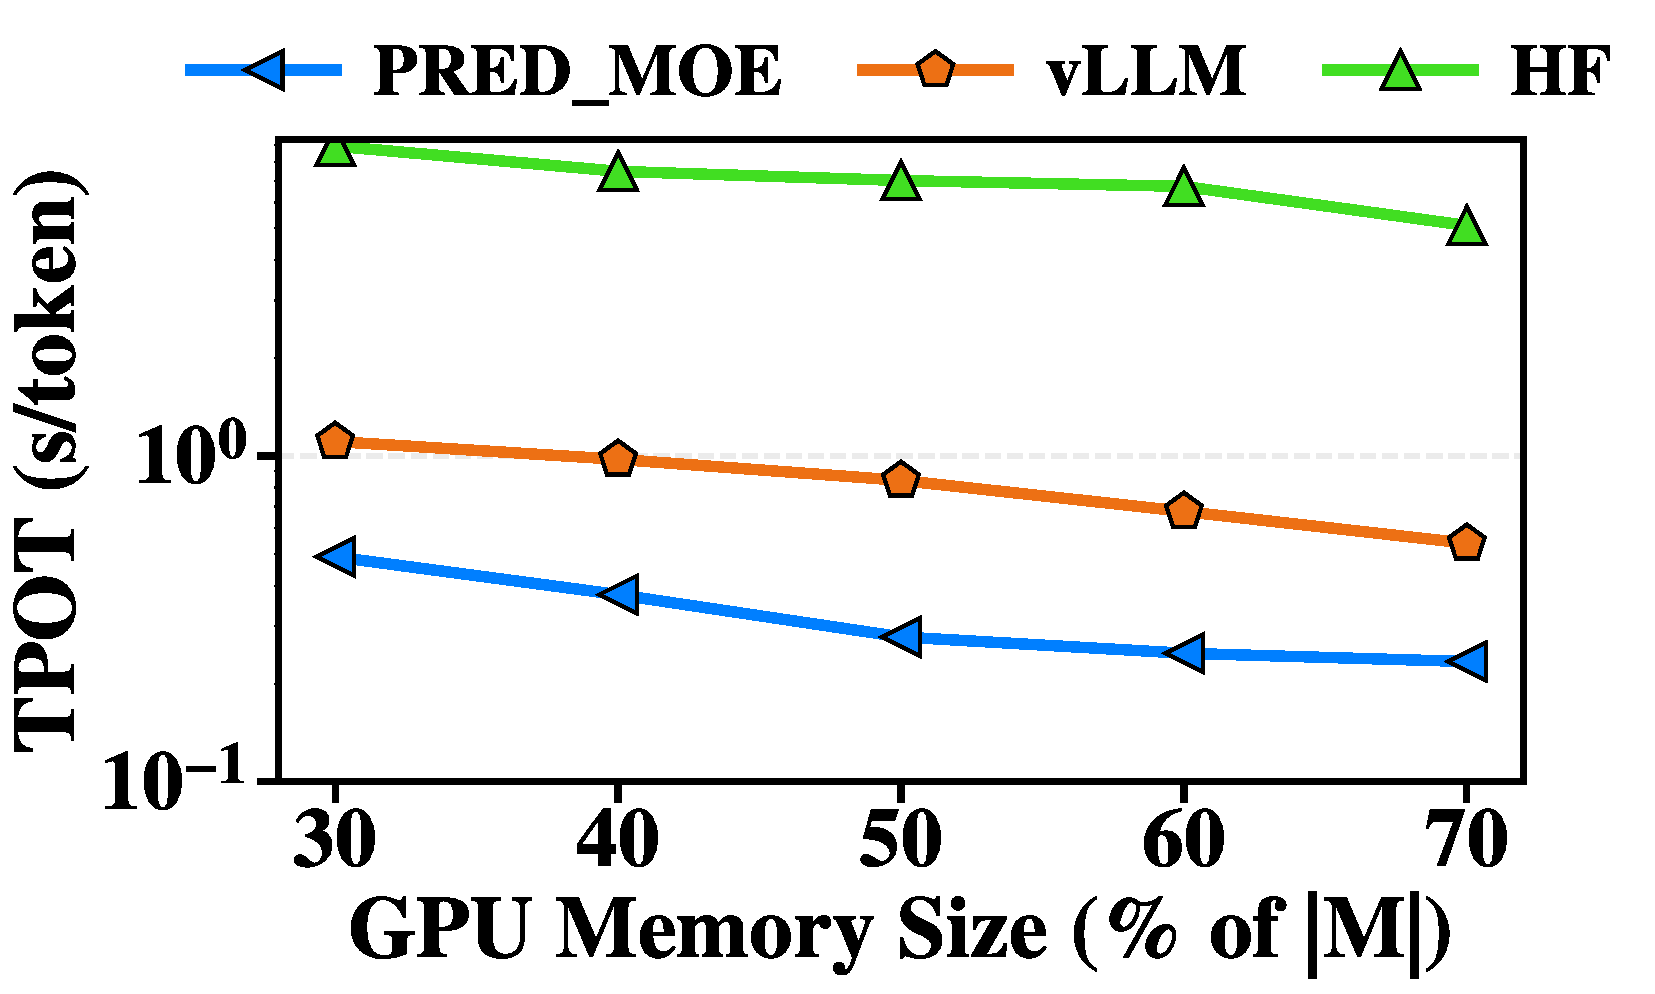
\includegraphics[width=\textwidth]{figures/poster_tpot_vs_gpu_memory.pdf}
        \end{center}
        \vspace{-0.1cm}
        }
        \label{subfig:tpot-vs-gpu-memory}
        \end{minipage}
    }
    %
    \hspace{-0.1cm}
    \subfigure[TPOT w.r.t. batch size]{
        \begin{minipage}[t]{0.475\linewidth}{
        \vspace{-0.00in}
        \begin{center}
        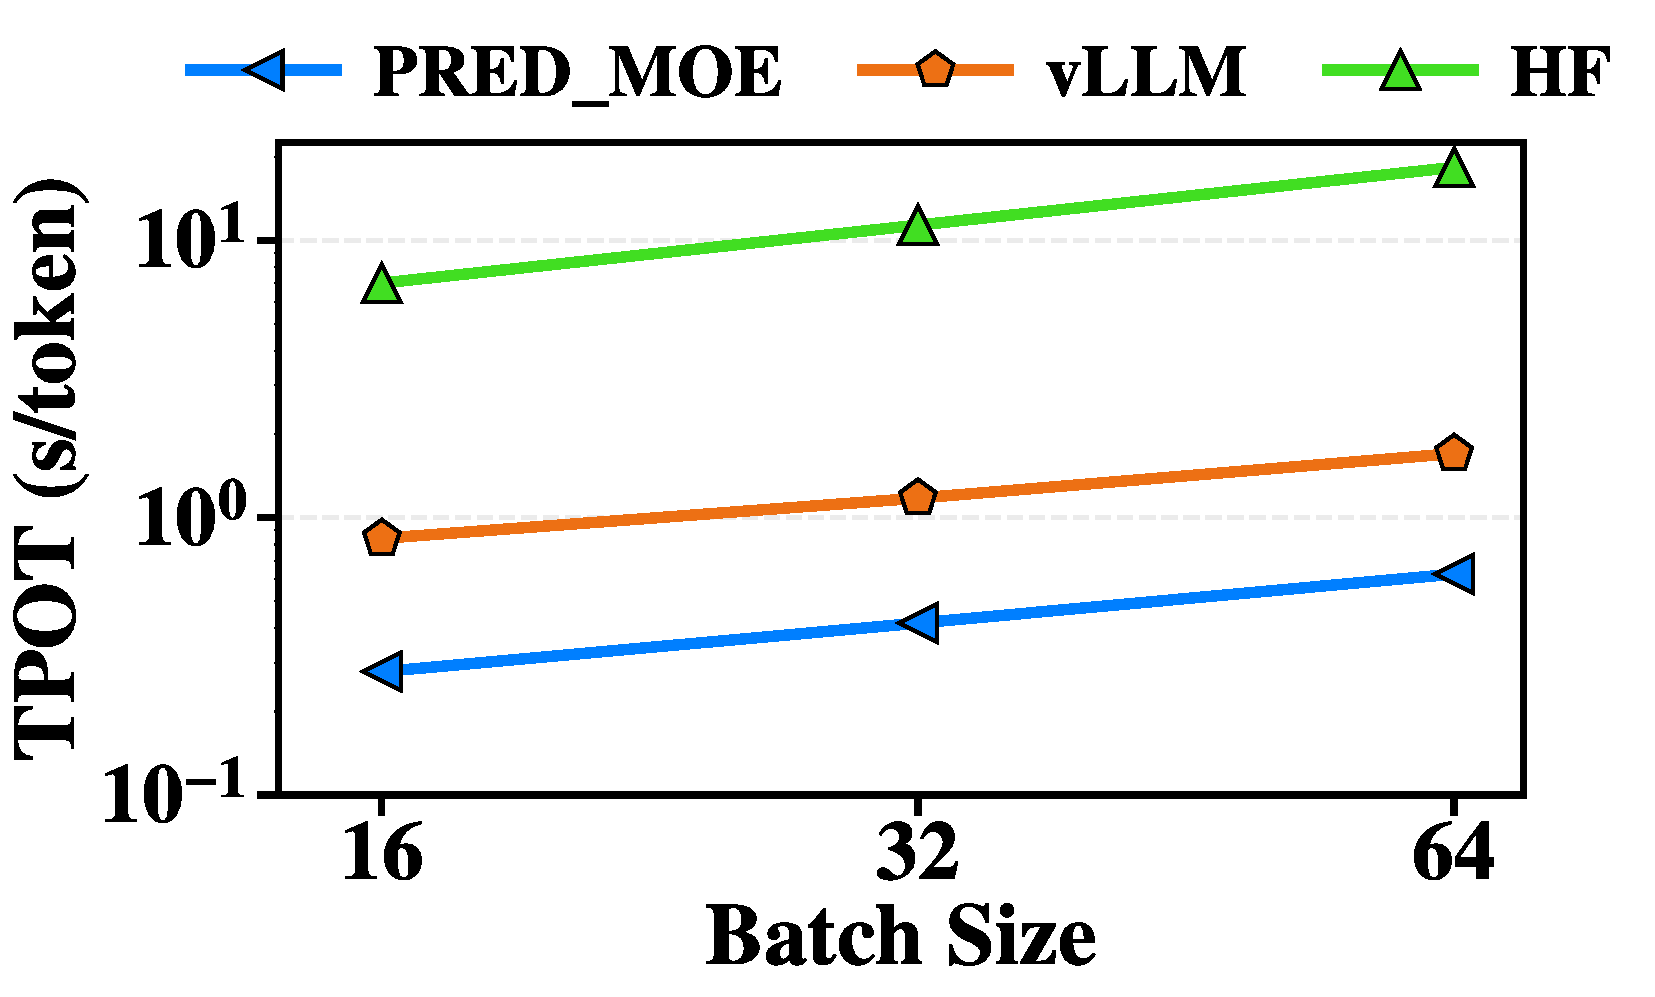
\includegraphics[width=\textwidth]{figures/poster_tpot_vs_batch_size.pdf}
        \end{center}
        \vspace{-0.1cm}
        }
        \label{subfig:tpot-vs-batch-size}
        \end{minipage}
    }

    \vspace{-0.2cm}
    \caption{\sysname's throughput in tokens per second (TPS) and TPOT in seconds per output token compared with vLLM and HF. In Figures (a) and (c), the batch size is $16$ requests and we vary the available GPU memory size relative to the model parameter size (${\sim}60 $GB for Qwen3-30B-A3B~\cite{yang2025qwen3, qwen2025qwen330ba3b}). In Figure (b) and (d) we fix the available GPU memory size as $30$GB and vary the batch size from 16 to 64.}
    \label{fig:performance-comparison}
    \vspace{-0.2cm}
\end{figure}

\smallskip
\subp{Evaluation setup.} In our preliminary evaluation, we use Qwen3-30B-A3B as the LLM foundation model, where each layer consists of $128$ experts and each token activates $K_l=8$ experts in each layer. We use MMLU-Pro~\cite{wang2024mmlupro, tigerlab2024mmluprodataset} as the dataset and we prompt the model to generate chain-of-thoughts before yielding the answer choice. Experiments were conducted on a server with 8 NVIDIA RTX 6000 Ada GPUs (48 GB GDDR6 each), each connected to the host CPU memory via PCIe 4.0 with 32 GB/s bidirectional bandwidth.

\smallskip
\subp{Training expert predictors.}
The expert predictors must be lightweight enough to run on the critical path without affecting generation speed. 
We therefore deliberately restrict both the predictors' architecture and their input features. 
The predictors are trained offline from traces collected during model execution on training data. Each trace records the generated token embeddings and the ground-truth routing logits, namely, the actual expert activations at every layer and decoding step. For each training example, we construct the lightweight predictor input from token embeddings at steps $t$ and $t-1$ together with the routing outputs at step $t-1$. The training target is the set of experts selected by the routers at the prediction horizon. Namely, we train two predictors targeting prediction horizon $h\in \set{0,1}$ denoted by $\mathcal{P}_{0+}$ that predict the activations for the current step $t$ and $\mathcal{P}_{1+}$ that predict the activations for the next step $t+1$.
Since each layer may activate multiple experts, we train the predictors using a multi-label objective over experts, applied independently at each layer. Concretely, the loss is the sum of per-layer binary cross-entropy terms between the predicted expert probabilities and the observed expert-activation indicators.
We implement each predictor using a small Transformer architecture of size $171$MB. 

\smallskip
\subp{\sysname policy at inference runtime.}
At the beginning of each step $t$, for each request $b\in\mathcal{B}_t$, the predictors output per-layer scores $s^h_{b,\ell,e}$, where $s^h_{b,\ell,e}$ is the softmax-normalized likelihood that expert $e$ will be activated at layer $\ell$ at step $t+h$.\footnote{Preliminary measurements show that running the predictors at inference adds less than $1\%$ end-to-end time overhead.}

For our initial prototype, we focus on eviction and utilize these scores to construct a three-phase policy. At the beginning of each step, the first phase computes, for each expert, two scores $p_{\ell, e, h=0}$ and $p_{\ell, e, h=1}$, which are the likelihoods of an expert being required at step $t+h$.\footnote{To construct these two scores, we use max-pooling across the batch dimension to obtain a total ordering of the experts, and then use this ordering to compute per-horizon priors $P_h($expert is actually active | predicted rank $r)$ and mapping back from rank to expert.}
The second phase aggregates the likelihood results across two horizons by $\bar{P}_{\ell, e} = p_{\ell, e, 0} + \lambda(1-p_{\ell, e, 0})p_{\ell, e, 1}$ where $\lambda \ge 0$ is fine-tuned during training to account for the reduced trustworthiness of prediction results at $h=1$ in comparison to $h=0$. Third, at layer $\ell$, upon a cache miss with the cache being full, \sysname initiates a CPU-GPU missing experts (i.e., $\mathcal{A}_{t,\ell}\setminus \mathcal{C}^{-}_{t,\ell}$) copy and evicts experts from its cache that have the lowest $\bar{P}$ score and are not in $\mathcal{A}_{t,\ell}$.
Preliminary measurements show that running the predictors during inference adds less than $1\%$ end-to-end time overhead.




\smallskip
\subp{End to end inference performance.} As Figure~\ref{fig:performance-comparison} indicates, \sysname achieves substantial improvement in both throughput in tokens-per-second (TPS) and inference latency in time-per-output-token (TPOT) over two state-of-the-art inference frameworks, namely, vLLM and Huggingface. 
Across different GPU memory sizes, \sysname improves over vLLM's and HuggingFace's TPS by $2.26 \sim 3.02\times$ and $18.23 \sim 25.18\times$ respectively; across different batch sizes, \sysname improves over vLLM's and HuggingFace's TPOT by $ 2.74 \sim 3.02\times$ and $18.23 \sim 28.62 \times$ respectively. Our analysis reveals that this improvement is mainly attributable to significantly reduced CPU-to-GPU copy traffic. For example, with a $16$-batch size and $50\%$ GPU memory, \sysname loads on average $\approx2.2\%$ of experts, while vLLM loads $\approx10.63\%$ and HF loads$\approx 50\%$. 

\begin{figure}[]
    \centering
    \vspace{0.1in}
    \hspace{-0.15cm}
    \subfigure[Recall rate $h=0$]{
        \begin{minipage}[t]{0.48\linewidth}{
        \vspace{-0.00in}
        \begin{center}
        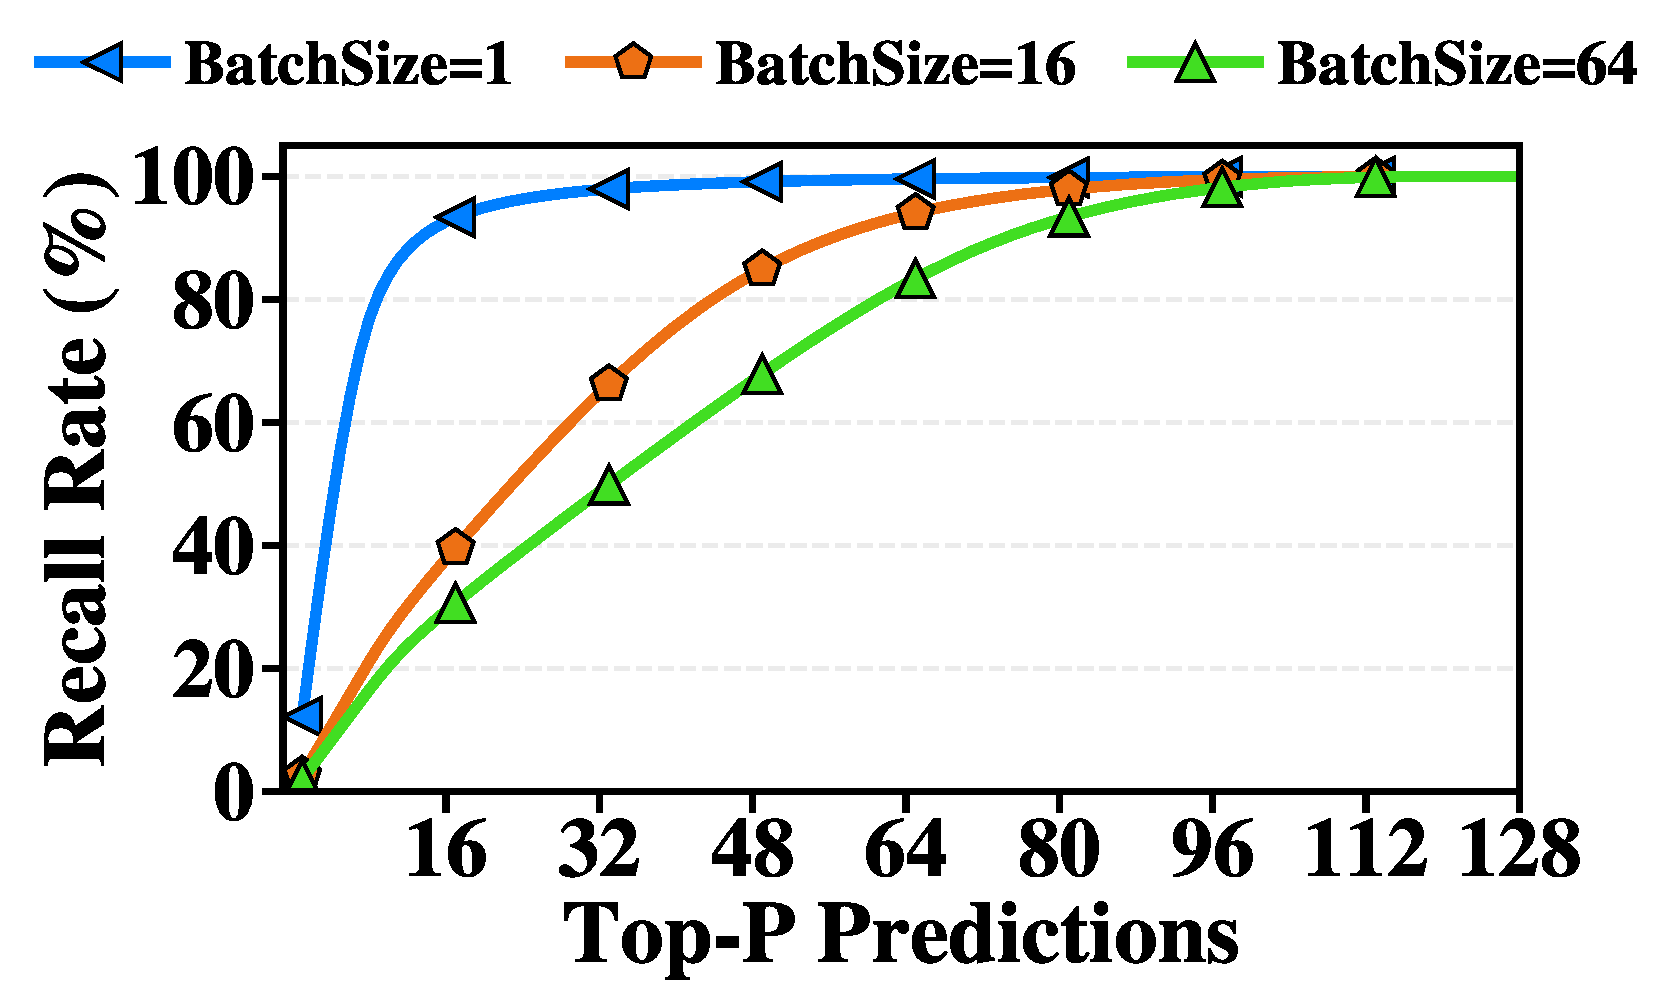
\includegraphics[width=\textwidth]{figures/poster_recall_vs_topk.pdf}
        \end{center}
        \vspace{-0.1cm}
        }
        \label{subfig:recall-vs-topk}
        \end{minipage}
    }
    %
    \hspace{-0.1cm}
    \subfigure[Recall rate $h=1$]{
        \begin{minipage}[t]{0.48\linewidth}{
        \vspace{-0.00in}
        \begin{center}
        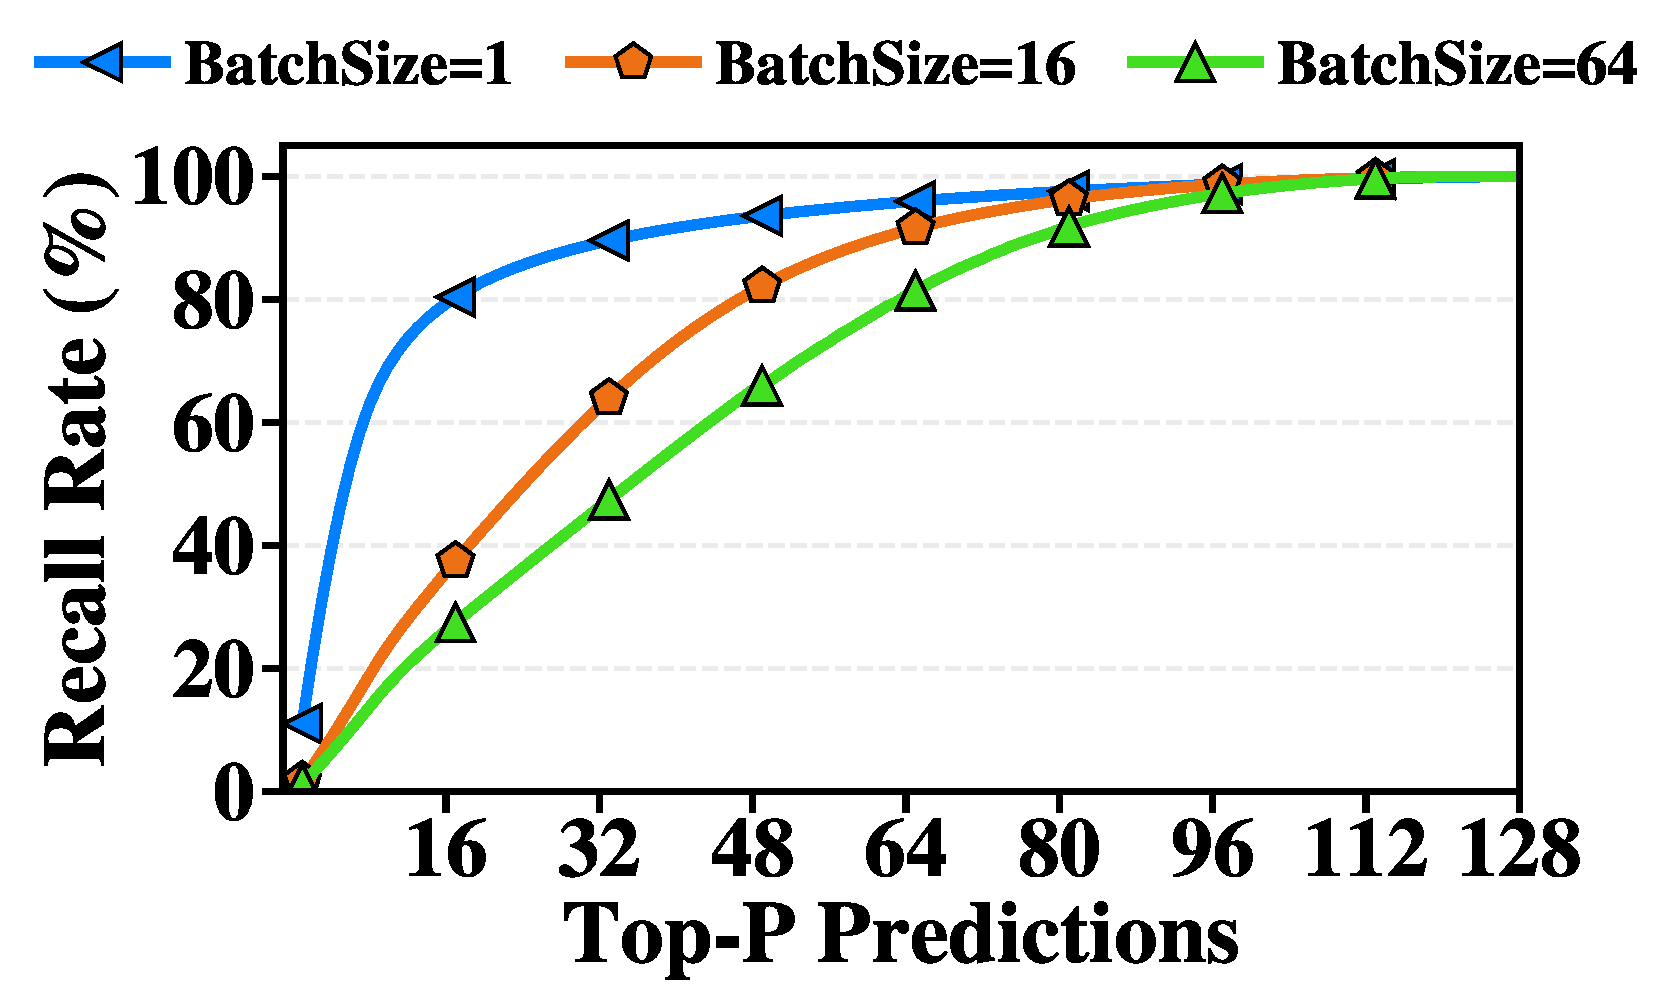
\includegraphics[width=\textwidth]{figures/poster_recall_vs_topk_h1.pdf}
        \end{center}
        \vspace{-0.1cm}
        }
        \label{subfig:recall-vs-topk-h1}
        \end{minipage}
    }

    \vspace{-0.5cm}
    \caption{The recall rate predicting the expert activation for horizons $h=0$ and $h=1$, varying the batch size.}
    \label{fig:prediction-recall}
\end{figure}

\smallskip
\subp{Predictor recall.} 
Figure~\ref{fig:prediction-recall} depict our predictors' recall which confirms our findings in Section \ref{sec:expert_activation_patterns}.
Interestingly, the amount of CPU-to-GPU loads, which bottleneck the end to end performance, with \sysname's policy, can be upper-bounded by the predictors' recall rate. 
Specifically, with a GPU memory capacity of $m\%$ model size and $h=0$, our eviction policy guarantees that the Top-$P=128*m\%$ experts that will be used in step $t$ will never be evicted. For example, the recall rate of $93.3\%$ at $P=64$ indicates that the amount of CPU-to-GPU copy is upper-bounded by $6.7\%$ of the total experts. 

\section{Future Work}
We plan to extend our prototype from prediction-guided eviction to a full prefetching-and-eviction system. This would require modeling not only cache misses, but also false prefetches, limited PCIe/NVLink and other interconnects bandwidth limitations and nonuniform networking expert-transfer costs. 

\bibliographystyle{ACM-Reference-Format}
\bibliography{reference}

\end{document}